\section{A Web Application for Optimization and Visualization}
\label{sec:web-app}
In order to make this optimization framework available to researchers, students, and anyone who would prefer not to work with the code itself, I developed a web application that implements its major components.
I developed this tool using the python library ``Streamlit", which facilitates the transformation of algorithms and visualizations to a web application.
Fortunately for the developer, coding in Streamlit web framework requires no handling of html, javascript, or other distractions.
Instead, Streamlit provides tools for converting Python code directly into interactive tables and plots.

This web application is initialize with a choice of three models and four data-sets (Figure \ref{fig:web-app-1}), although it would be straight-forward to add additional ones.

\begin{figure}
\begin{center}
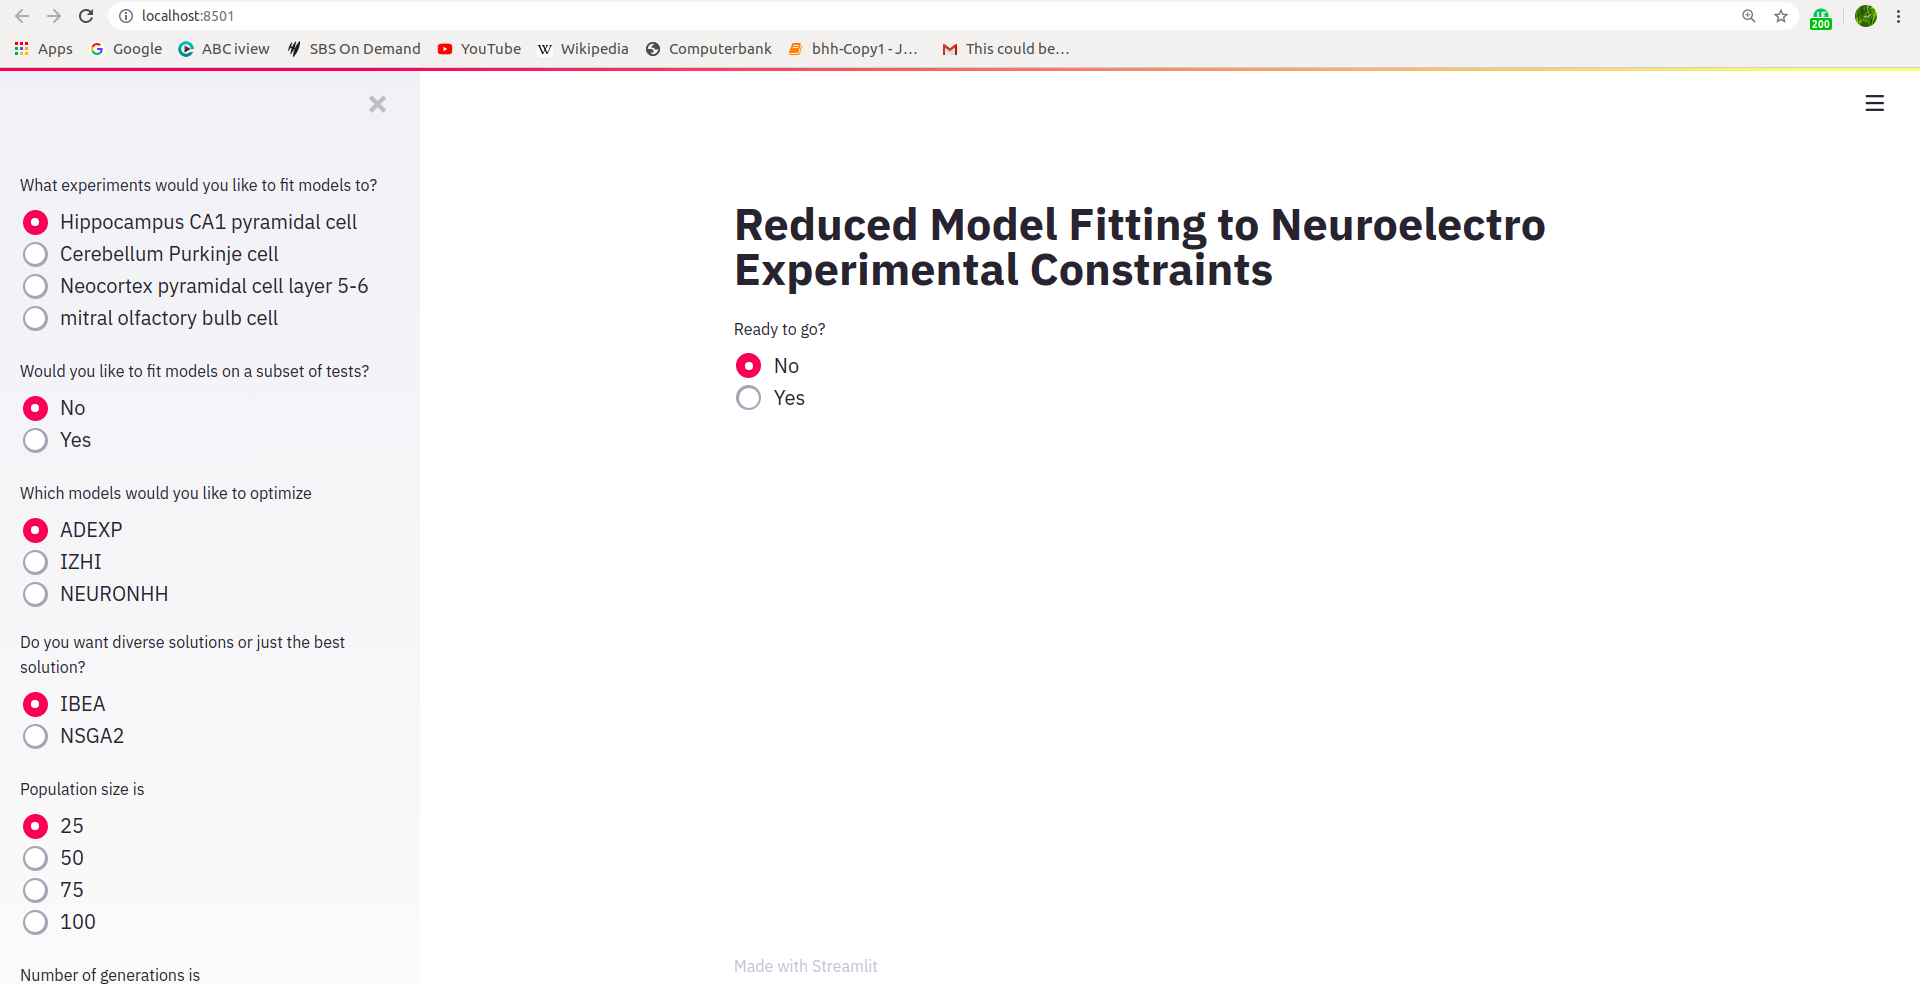
\includegraphics[scale=1]{chapters/app_tex/web_app_thesis}
\caption[Web application (1)]{The side-pane of the web application provides users with a choice of three models, and four data sets that can be used to fit data.
}
\end{center}
\label{fig:web-app-1}
\end{figure}

The user is given a choice of optimization parameters (for example, the number of chromosomes or the number of generations), and shown the experimental data that will be used to guide the optimizer (Figure \ref{fig:web-app-2}).

\begin{figure}
\begin{center}
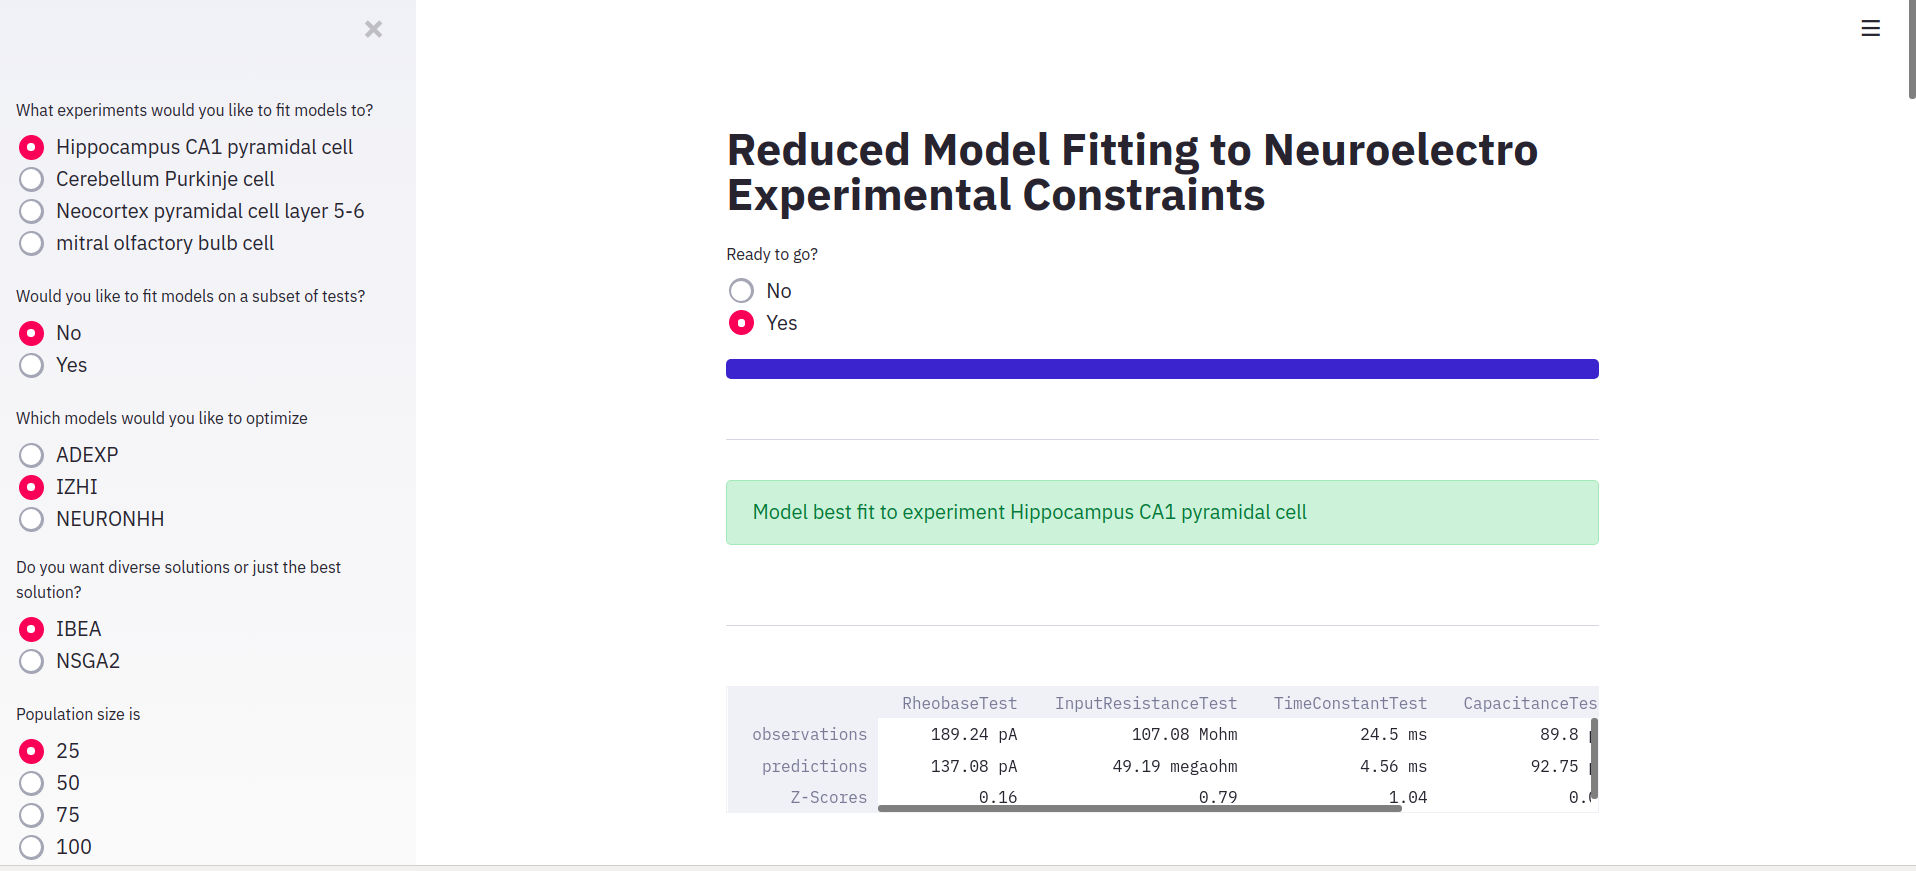
\includegraphics[scale=1]{chapters/app_tex/app_results}
\end{center}
\caption[Web application (2)]{The Optimizer has completed a job fitting to neuro-electro data,  an agreement table is shown to the user, and optionally the user can scroll down through a visualisation of model fitness metrics, such as the $\chi^{2}$ test value. They can inspect interactive model waveforms and they can also download the pickled model}
\label{fig:web-app-2}
\end{figure}

When optimization is complete the user is shown the parameters of the optimized model as well as key membrane potential traces (i.e. response to the rheobase current injection) for inspection (Figure \ref{fig:web-app-3}.

\begin{figure}
\begin{center}
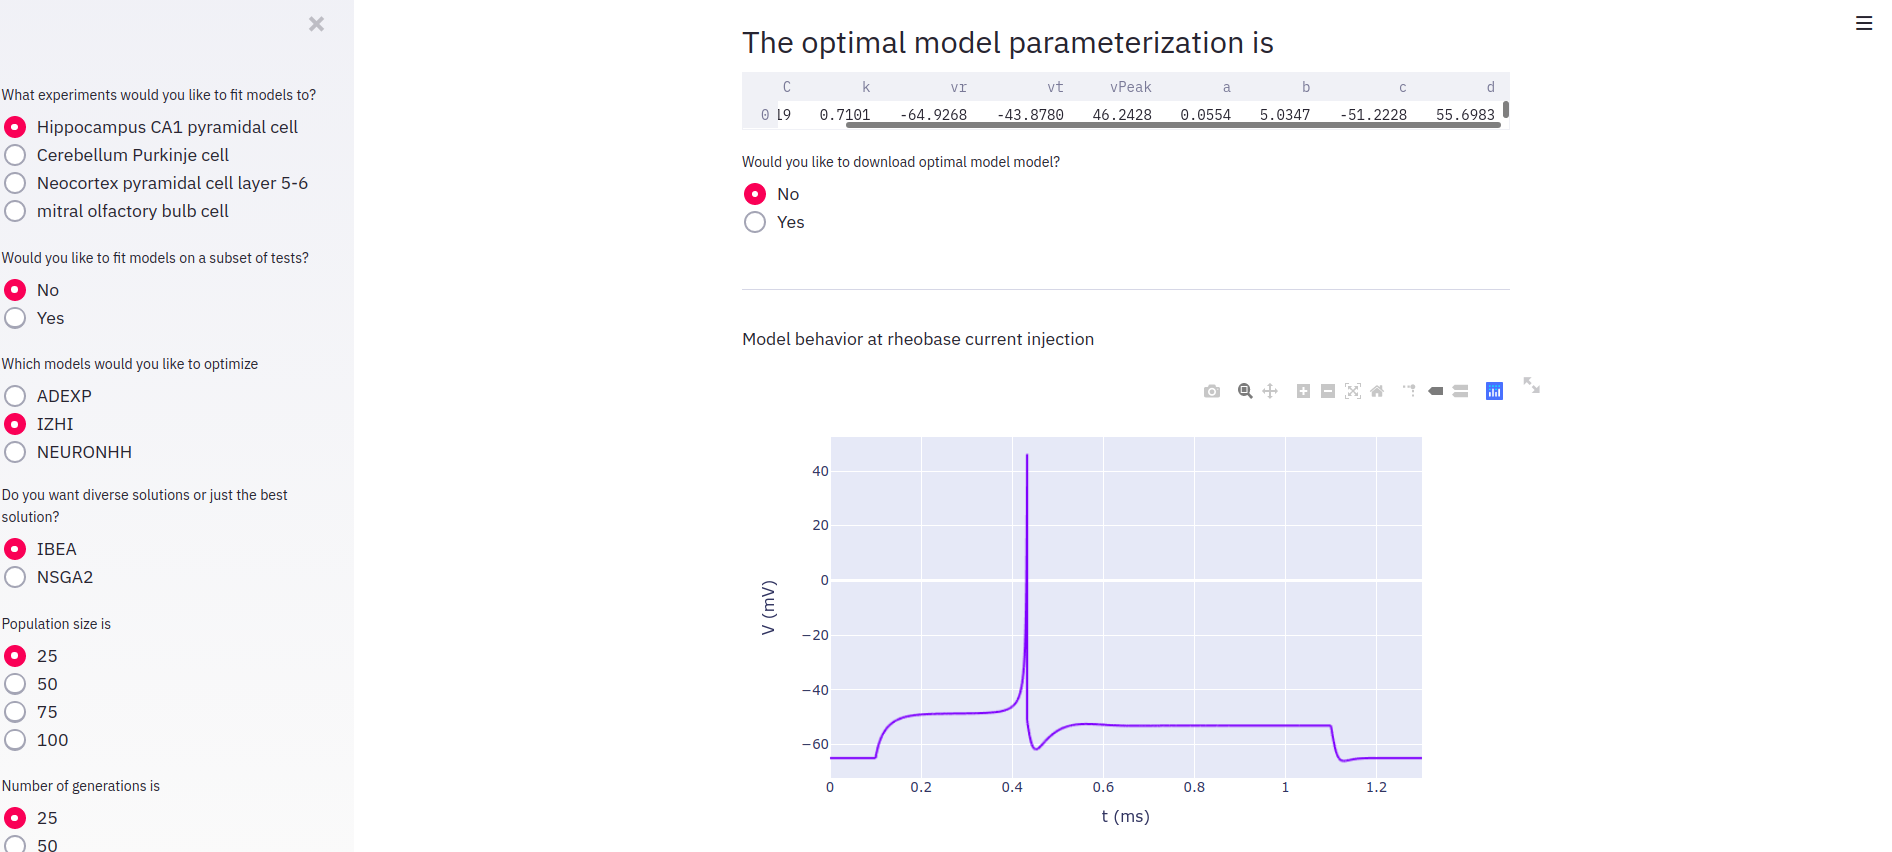
\includegraphics[scale=1]{chapters/app_tex/more_app_results}
\end{center}
\caption[Web application (3)]{An accompanying interactive visualisation of the optimized model neuron firing under rheobase firing, and also under passive conditions is supplied.}
\ref{fig:web-app-3}.
\end{figure}

Finally, the user is shown the $\chi^{2}$ statistic (and p-value) for the optimized model, and provided with a link is provided to download these parameters for their own use (Figure \ref{fig:web-app-4}.
Future work will allow the user will be able to download a NeuroML file of the optimized model.

\begin{figure}
\begin{center}
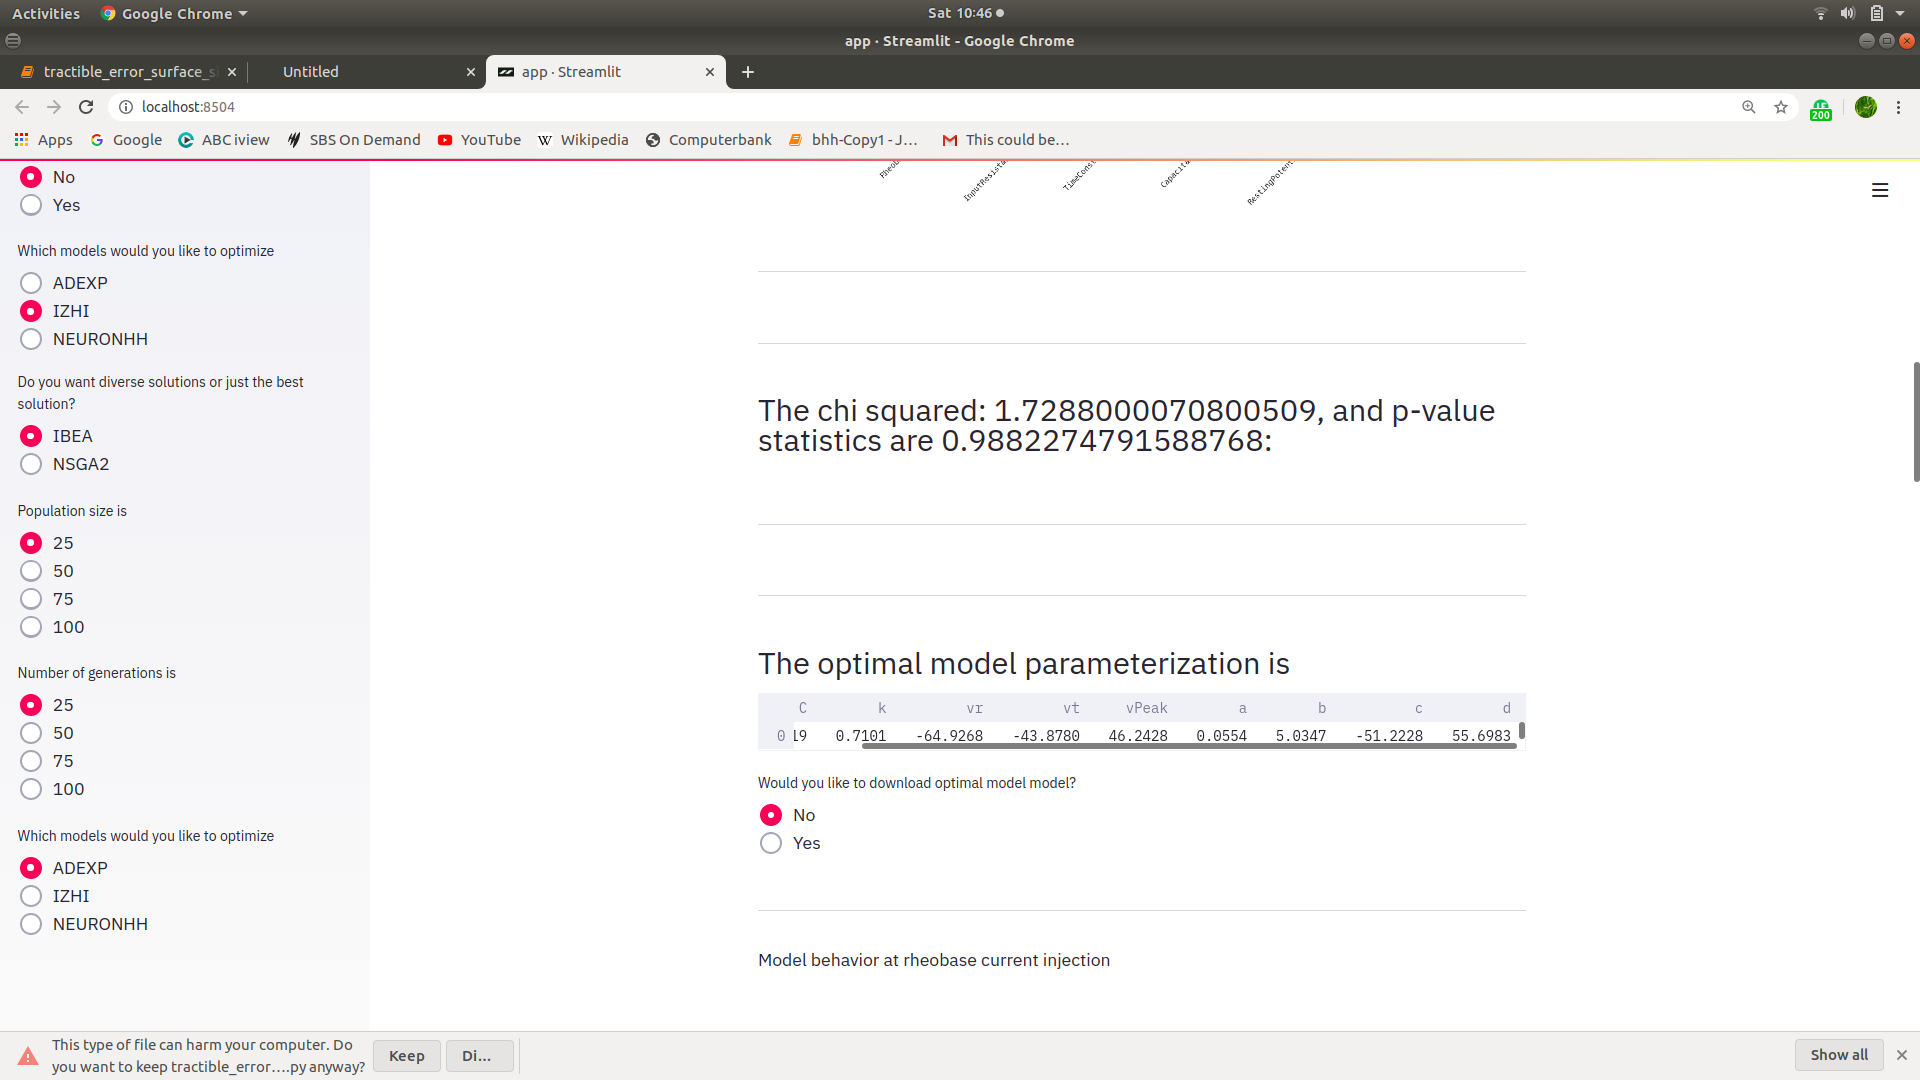
\includegraphics[scale=1]{chapters/app_tex/Screenshot from 2020-09-19 10-46-32}
\end{center}
\caption[Webapp prompt to download optimized model]{The Webapp can respond to a prompt to download an optimized version of a model, this feature has been flagged to support the download of a NeuroML version of the model}
\ref{fig:web-app-4}.
\end{figure}

Because some of the details of the scoring associated with optimization are unfamiliar to most people, another visualization is provided (Figure \ref{fig:web-app-5} which helps the user visualize the meaning of a Z-score in an optimization context, and displays this information for each feature used to constrain the optimization.
Additional information about the stimuli used and the time taken to run the simulations are also provided.

\begin{figure}
\begin{center}
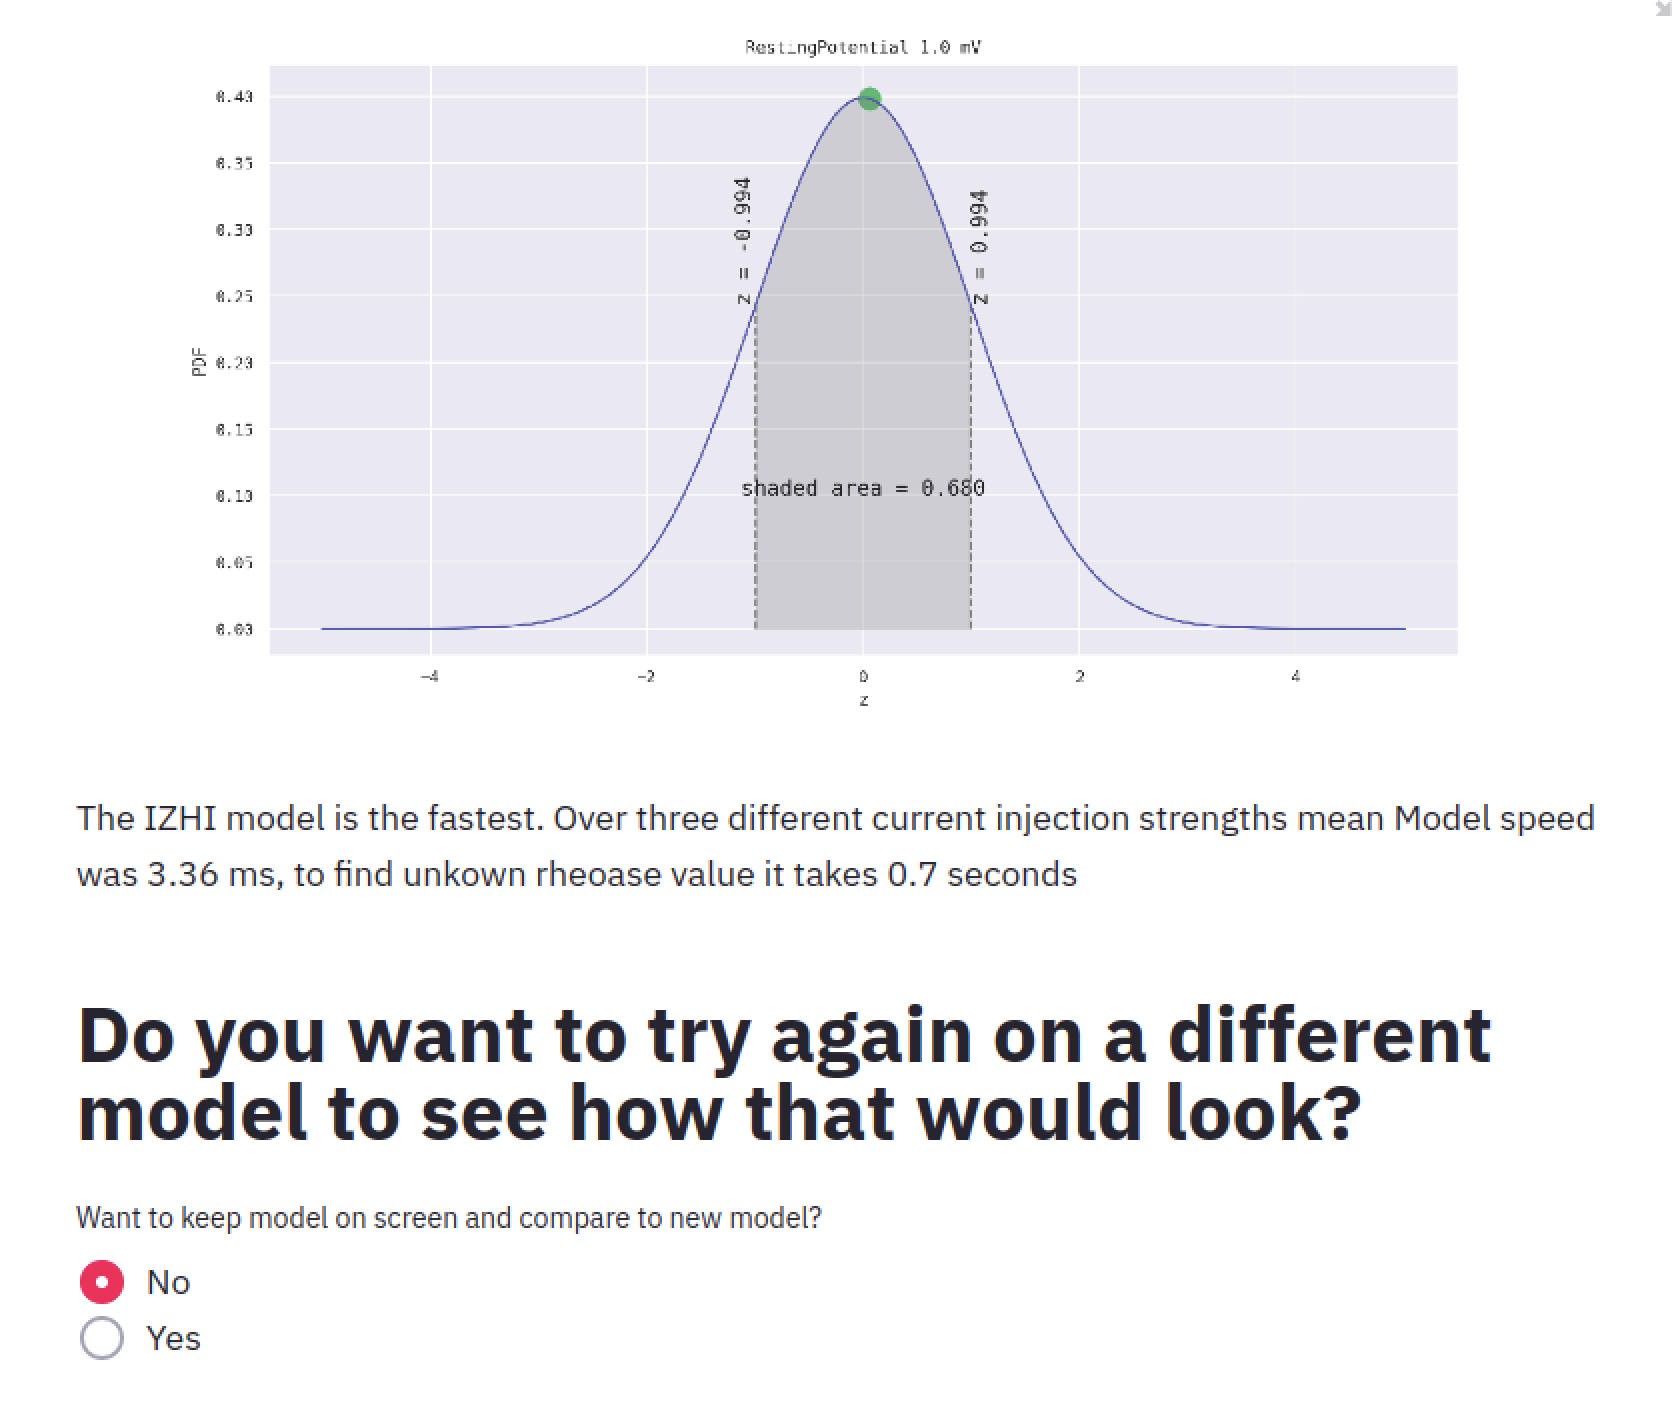
\includegraphics[scale=1]{figures/fixed_white_space.png}
\caption[Web application Z-score view]{In principle the web application is compatible with the approach of fitting models to the supra threshold multi-spiking experiments approach but this functionality does not exist at the time of writing}
\end{center}
\end{figure}
